\documentclass[conference]{IEEEtran}
% \IEEEoverridecommandlockouts
% The preceding line is only needed to identify funding in the first footnote. If that is unneeded, please comment it out.
\usepackage{cite}
\usepackage[portuges,brazil,english]{babel}
\usepackage{amsmath,amssymb,amsfonts}
\usepackage{algorithmic}
\usepackage{graphicx}
\usepackage{textcomp}

% pacotes que não estavam no modelo original:
\usepackage[pagebackref=true,breaklinks=true,colorlinks,bookmarks=false]{hyperref}
\usepackage{dirtree}
\usepackage{subfig}

\def\BibTeX{{\rm B\kern-.05em{\sc i\kern-.025em b}\kern-.08em
    T\kern-.1667em\lower.7ex\hbox{E}\kern-.125emX}}
\begin{document}

%%%%%%%%%%%%%%%%%%%%%%%%%%%%%%%%%%%%%%%%%%%%%%%%%%%%%%%%%%%%%%%%
% \title{Transfer Learning Between Different Games\\via Generative Models}
\title{Fish tracker 3D\\for State-to-Action Mappings}

\author{ 
    \IEEEauthorblockN{Tiago Petená Veraldi}
    \IEEEauthorblockA{187700\\t187700@dac.unicamp.br}
    \and
    \IEEEauthorblockN{Henrique Machado Gonçalves}
    \IEEEauthorblockA{169621\\h169621@dac.unicamp.br}
}

\maketitle

%%%%%%%%%%%%%%%%%%%%%%%%%%%%%%%%%%%%%%%%%%%%%%%%%%%%%%%%%%%%%%%%
\begin{abstract}
In this work we used the ORB(oriented fast and rotated brief)\cite{orb} algorithm to track 3d movement of fishes from 2 views of an aquarium based on the “3D Zebrafish Tracking Benchmark Dataset”\cite{zbfish}
. This is a challenging problem as the fishes are very similar, can be occluded and have unpredictable movement with the naive approach we took. 

We managed to track the fish with the help of their ground-truth box location but much work is still needed to get a somewhat reliable tracking.
 
\end{abstract}


%%%%%%%%%%%%%%%%%%%%%%%%%%%%%%%%%%%%%%%%%%%%%%%%%%%%%%%%%%%%%%%%
% Introduction: This section introduces your problem, and the overall plan for approaching your problem

\section{Introduction}\label{sec:intro}
\subsection{Project Overview}
% The introduction and motivation of the work. 
 
\begin{figure}[h]
    \centering
    \fbox{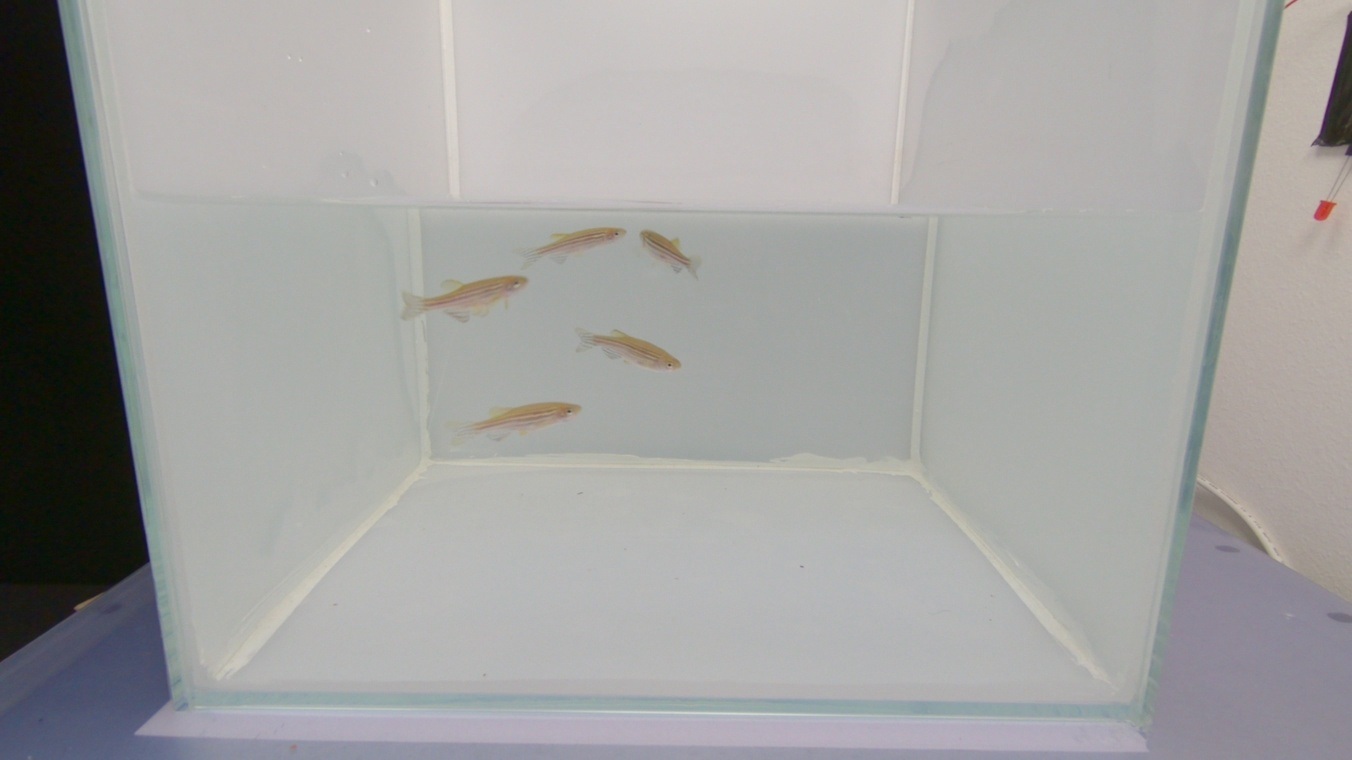
\includegraphics[width=0.46\textwidth]{imgs/000106.jpg}}
    \caption{Zebrafish aquarium front view.}
    \label{fig:fish}
\end{figure}

 Three-dimensional object tracking mimics the well-studied image-based 2D detection but comes with additional challenges. Objects in a 3D world do not follow any particular orientation, box-based detectors have difficulties enumerating all orientations, so we use a key-point detector to find the objects, size and their orientation in the 3D world. 3D object tracking simplifies to greedy closest-point matching and creating descriptors to create a model based on the ground truth based in a short frame window. Developing accurate system giving less attention to practical considerations such as computational cost and system complexity may diverge from a real time application. However, the implementation proposed is based on a rather naive model fitting, predicting the trajectory based on this model can be very forgiven due the lack of robustness as they compared to the results from other works. 


With the project description, we started implementing our application based with a mixture of template matching with key-point descriptors, however, due to problems in the workflow we were not able to actually complete the full task proposed in this project.

% FIXME falar que geramos as trajetórias (colocar p.e. o tamanho/qtd. de arquivos)

\subsection{Interest Points and Descriptors}
The ORB(Oriented Fast and rotated brief) algorithm was chosen due to it's speed, as it performs as well as SIFT on the task of feature detection while being orders of magnitude faster.  This method uses a rotational invariant version of Fast and works by, given a pixel p in an array, comparing the brightness of it's surround 16 pixels, a small circle around. Pixels in the circle is then sorted into three classes - lighter, darker or similar to p. If more than 12 pixels are darker or brighter than p than it is selected as a keypoint. The keypoints found give us information of the location of determining edges in an image. These are then filtered by the ones with the n highest harris-corner responses. However, FAST features do not have an orientation component and multiscale features. So ORB uses a multiscale image pyramid. An image pyramid is a multiscale representation of a single image, that consist of sequences of octaves all of which are versions of the image at different resolutions. Each octave is a downscale version of the image than the previous layer. Once we create the pyramid the ORB uses the FAST algorithm to detect keypoints in the image. By using this method at each layer, ORB is effectively locating keypoints at different scale, in this way is partial scale invariant.

\begin{figure}[h]
    \centering
    \fbox{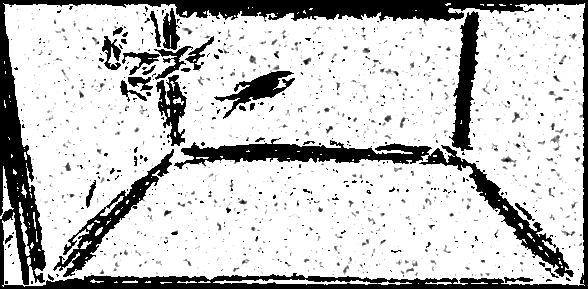
\includegraphics[width=0.46\textwidth]{imgs/harriscorner.png}}
    \caption{Harris Cornerness response used to filter keypoints given by the FAST algorithm.}
    \label{fig:harris}
\end{figure}

After locating keypoints, now we assign an orientation to each keypoint based where they are facing depending on how the levels of intensity change around that neighborhood. For detecting intensity change, we use intensity centroid. The centroid assumes that a corner's intensity is offset from its center, ant this vector may used to imply an orientation. Then we apply the Brief(Binary robust independent elementary feature) algorithm.

Brief take all keypoints found by the fast algorithm and convert in into a binary feature vector so that together they can represent a object. In order to prevent the descriptor from being too sensitive to high-frequency noise every image created in the pyramid is smoothed using a Gaussian kernel. The defined neighborhood around pixel was based on a pre-trained model, instead of using a random pair of pixels. The first pixel in the pair is drawn form a Gaussian distribution centred arround the fist pixel with a standard deviation. Selecting the pairs based in the model we assign the value to then and repeat this process 256 times for each keypoint. Brief create a vector for each keypoint in a image. However, Brief also isn't invariant to rotation so we use rBrief (Rotation-aware BRIEF) trying to add orientation functionality, without losing out on the speed aspect of Brief. ORB proposes a method to steer BRIEF according to the orientation of the keypoints. Than it discretizes the angle to increments of 2$\pi$/30 (12 degrees), and construct a lookup table of precomputed BRIEF patterns. As long as the keypoint orientation is consistent across views.  

\subsection{Tracking and Matching}
The ground truth boxes given by the Dataset were used to create models of each fish containing it`s keypoints and descriptors, while removing unwanted keypoints from aquarium edges and debris. These models loose accuracy as there is a lot of occlusion from the fishes, but provide a way to track the fishes with the help of the boxes.

These could be used in feature matching, providing a way to dismiss the need of the fish location information. This was not implemented in this project.
\begin{figure}[h]
    \centering
    \fbox{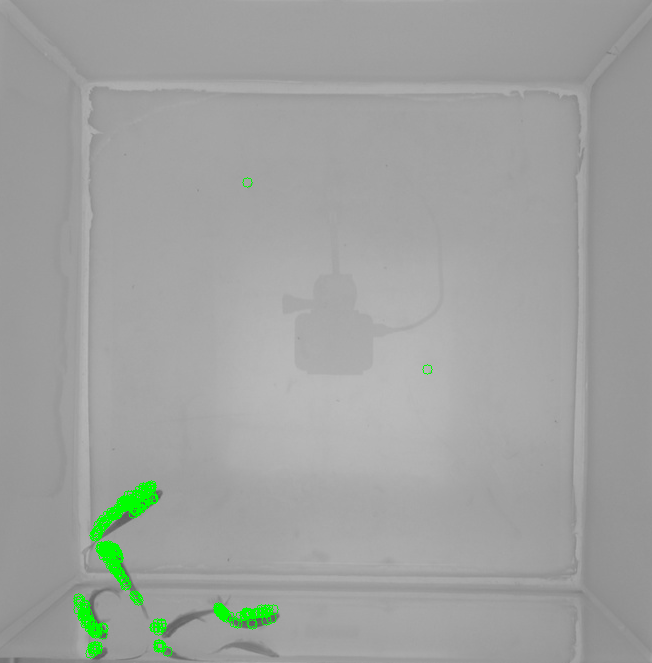
\includegraphics[width=0.46\textwidth]{imgs/top_kp_screenshot_13.11.2020.png}}
    \caption{Located keypoints from top view.}
    \label{fig:topview}
\end{figure}
\begin{figure}[h]
    \centering
    \fbox{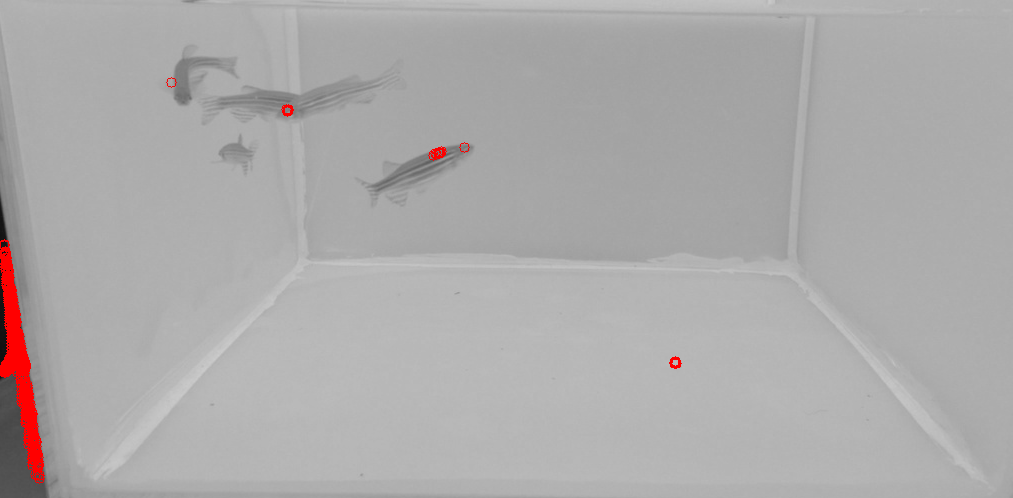
\includegraphics[width=0.46\textwidth]{imgs/front_kp_screenshot_13.11.2020.png}}
    \caption{Located keypoints from front view.}
    \label{fig:frontview}
\end{figure}

\begin{figure}[h]
    \centering
    \fbox{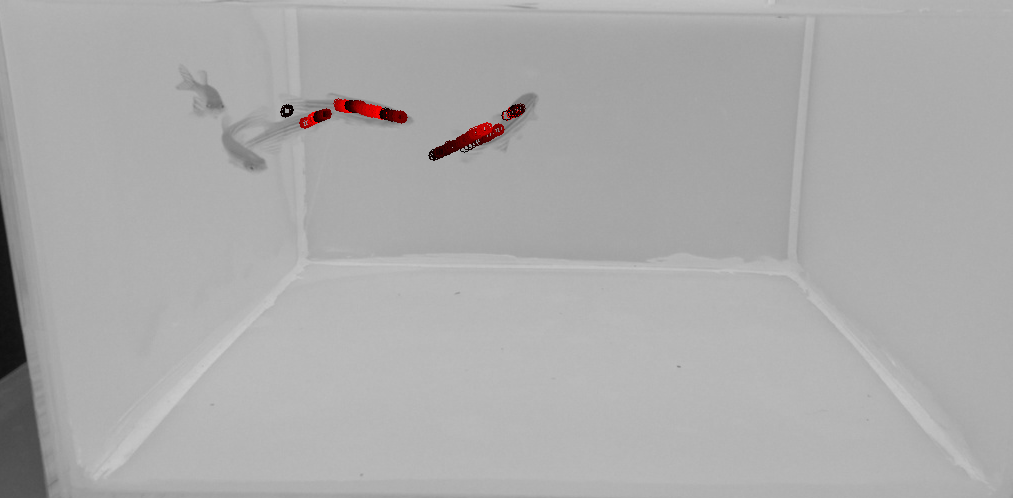
\includegraphics[width=0.46\textwidth]{imgs/fishtime.png}}
    \caption{Front view fish tracking.}
    \label{fig:fishloc}
\end{figure}

%%%%%%%%%%%%%%%%%%%%%%%%%%%%%%%%%%%%%%%%%%%%%%%%%%%%%%%%%%%%%%%%
\section{Conclusions and Future Work}
%  Conclusion: What have you learned? Suggest future ideas.
% The main conclusions of the work as well as some future directions for other people interested in continuing this work. 

Feature tracking and description is already a big challenge by itself. We were able to implement the ORB algorithm successfully despite the short window of time and an unexpected class drop from a group member. This has made possible tracking the 3d position of multiple fishes with the help of object-detection like boxes. 

Future work could encompass, while finishing the entire project proposal, optimizing the calculation of the ORB pyramids and the BRIEF feature description calculations. Learning based algorithms could be used to predict fish movement and minimize the occlusion problem.



%%%%%%%%%%%%%%%%%%%%%%%%%%%%%%%%%%%%%%%%%%%%%%%%%%%%%%%%%%%%%%%%
\bibliographystyle{IEEEtran}
\footnotesize{\bibliography{main}}
\noindent {\small{Links accessed on November 2020.}}

\end{document}
